\documentclass[../diploma.tex]{subfiles}
\begin{document}\label{sec:2}
\graphicspath{ {../images/} }

Данная глава, центральная часть этой работы, посвящена алгоритмическому описанию различных стратегий вычисления, которые будут применяться для упрощения системы уравнений. Сначала будут описаны простейшие нативные стратегии, затем они будут усложняться добавлением новых эвристик и оптимизаций. Отдельно будет описана работа с условными операторами, порождающими несколько веток вычисления.

\subsection{Анализ входных данных}\label{analysis}

\begin{wrapfigure}{l}{0.25\textwidth}
    \centering
    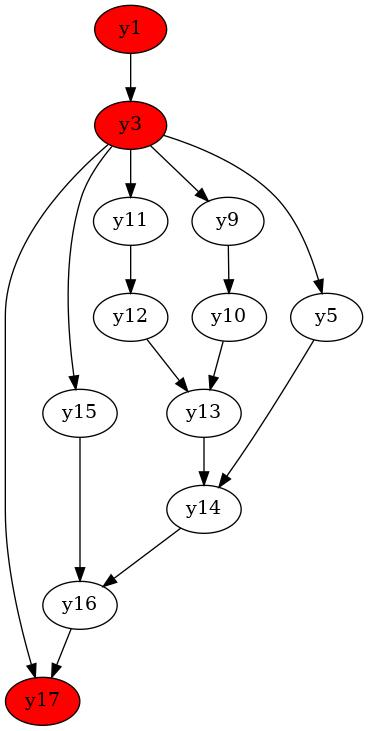
\includegraphics[width=0.25\textwidth]{graph_simple1.jpeg}
    \caption{Графовый вид простейшей системы}\label{graph_simple1}
\end{wrapfigure}

В предыдущей главе было описаны два принципиально отличающихся порядка вычисления: нормальный (в Coq тактика \texttt{lazy}) и аппликативный (в Coq тактика \texttt{cbv}) порядки, а также приведены их существенные недостатки. Рассмотрим, применимы ли эти недостатки к изучаемой задаче.

Основной недостаток аппликативного порядка --- неэффективная работа с "мёртвым кодом", блоками кода, результат редукции которых не влияет на итоговое вычисление. Могут ли такие блоки кода присутствовать во входных данных? Напомним, что входные данные состоят из набора уравнений $y_i = T_i$ и спецификации $P(y_0, y_n)$. Спецификация $P$ формально может быть любым предикатом, однако на практике в каждом конкретном доказательстве верификатора интересуют только некоторый срез системы, поведение отдельных частей программы. Из этого следует, что те части программы, которые не относятся к верифицируемому свойству, в терме $P(y_0, y_n)$ как раз и окажутся "мёртвым кодом". Вдобавок, при определённых стартовых состояниях $y_0$ некоторые ветки кода, отражённые в последующих уравнениях $y_i = T_i$, могут оказаться нерелевантными. К примеру, верификатора интересуют только стартовые состояние, при которых некоторое булевое поле равно \texttt{true}, тогда \texttt{else}-ветки соответствующих условных операторов окажутся мёртвым кодом. Таким образом, недостатки аппликативного порядка применимы к этой задаче в полной мере.

Основным недостатком же нормального порядка (особенно версии без мемоизации) является дублирование работы при преждевременной подстановке аргументов. Поскольку определение рассматриваемой системы уравнений разрешает в $T_i$ использовать любые $y_j$ для $j < i$, такое дублирование в теории может быть значительным. Чтобы изучить свойства реально рассматриваемых систем, был разработан графовый визуализатор. На рисунке \ref{graph_simple1} представлен графовый вид системы уравнений, построенной по простейшему линейному блоку кода (тест из множества Simple при n = 1, подробнее см. в разделе \ref{dataset}). Ребро $y_i \rightarrow y_j$ означает, что в $T_j$ используется $y_i$, а красным выделены вершины, соответствующие глобальным состояниям системы. Заметим, что поскольку $T_j$ не может ссылаться на $y_i$, если $j \le i$, то граф является ациклическим ориентированным графом. 

\begin{wrapfigure}{l}{0.25\textwidth}
    \centering
    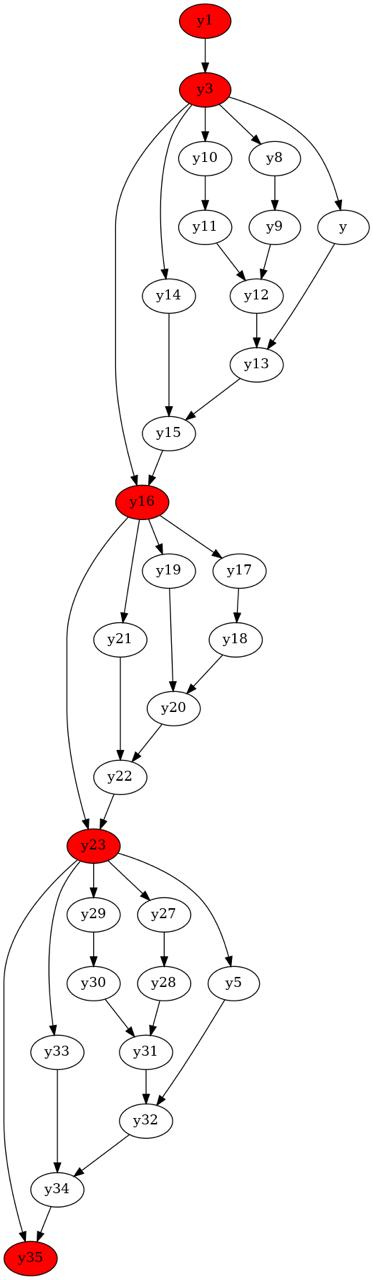
\includegraphics[width=0.25\textwidth]{graph_simple2.jpeg}
    \caption{Графовый вид системы из двух блоков кода}\label{graph_simple2}
\end{wrapfigure}

Если бы этот граф имел вид "бамбука", то есть если бы исходящая и входяшая степень каждой вершины была бы не больше одного, то можно было бы заключить, что нормальный порядок подходит отлично, так как подстановка не дублирует работу и мемоизация не требуется. Однако даже на простейшем линейном коде наблюдается достаточно ветвистый граф. А именно, существуют пять различных путей из $y_3$ в итоговое состояние $y_{17}$, то есть в худшем случае работа по редукции $y_3$ будет продублирована пять раз. Отметим, что $y_3$ соответствует глобальному состоянию системы, то есть является относительно большим термом, и дублирование его редукции даже несколько раз нежелательно.

На рисунке \ref{graph_simple2} представлен граф, построенный на основе двух блоков кода из предыдущего примера, с небольшой соединительной конструкцией между ними (тест из множества Simple при n = 2). Этот граф иллюстрирует, что число путей из стартовой вершины в итоговую, а значит, и потенциальное дублирование работы, становится экспоненциальным при увеличении размеров кода. Напомним, что код для этих иллюстраций взят упрощенный, на реальных примерах, особенно с разветвлением кода по условным операторам дублирование может быть ещё сильнее. Таким образом, при выборе нормального порядка необходима мемоизация, иначе замедление будет экспоненциальным, что недопустимо.

Итак, оба подхода имеют свои недостатки, и предварительный анализ входных данных показывает, что для рассматриваемой задачи оба недостатка --- "мёртвый код" и дублирование при подстановке --- применимы в полной мере. Дублирование при подстановке частично решается мемоизацией, однако эта техника создаёт определённые накладные расходы, и до перехода к экспериментам неочевидно, будет ли эти расходы стоить оптимизации по "мёртвому коду" по сравнению с аппликативным порядком. Соответственно, при дальнейшей разработке стратегий будут использоваться оба порядка и идеи, связанные с каждым из них.

\subsection{Базовые стратегии}

Прежде чем приступить к разработке стратегий, заметим, что можно исключить из рассмотрения все уравнения, которые в итоге не используются в $P$, тем самым избавившись от "мёртвого кода" на уровне уравнений. Это можно сделать эффективно (по отношению к остальной работе), применив следующий трюк: поскольку встроенная тактика \texttt{clear} упадёт, если какой-то элемент контекста где-то используется, последовательным применением этой тактики можно найти неиспользуемые элементы. В дальнейшем будем считать, что все $y_i$ транзитивно задействованы в $P$.

Первой рассматриваемой стратегией является простая стратегии \texttt{native}, включающая в себя только один запуск редукции. Приведём набор уравнению к \textit{let-форме}, то есть воспользуемся конструкцией \texttt{let} внутреннего языка Coq и преобразуем каждое уравнение $y_i = T_i$ в часть единого терма \texttt{let} $y_i = T_i$ \texttt{in} $\dots$, а после всех \texttt{let-in} конструкций вставим верифицируемое свойство $P$. Получив из входных данных единый терм, редуцируем его с помощью нативных редукций \texttt{lazy} или \texttt{cbv}.

\begin{megaalgorithm}\captionsetup{labelfont={sc,bf}, labelsep=newline}
    \caption{native-lazy}
  \begin{algorithmic}
    \State $(Y, P)\gets$ input
    \State $F(x) \gets x$
    \For{$i \gets 1$ to $|Y|$}
        \State $F(x) \gets F($\texttt{let} $x_i = T_i$ \texttt{in} $x)$
        \For{$j \gets i + 1$ to $|Y|$}
            \State $T_j \gets T_j[y_i := x_i]$
        \EndFor
    \EndFor
    \State \Return {$lazy(F(P))$}
  \end{algorithmic}
\end{megaalgorithm}  

\begin{megaalgorithm}\captionsetup{labelfont={sc,bf}, labelsep=newline}
    \caption{native-cbv}
  \begin{algorithmic}
    \State $(Y, P)\gets$ input
    \State $F(x) \gets x$
    \For{$i \gets 1$ to $|Y|$}
        \State $F(x) \gets F($\texttt{let} $x_i = T_i$ \texttt{in} $x)$
        \For{$j \gets i + 1$ to $|Y|$}
            \State $T_j \gets T_j[y_i := x_i]$
        \EndFor
    \EndFor
    \State \Return {\textcolor{red}{$cbv(F(P))$}}
  \end{algorithmic}
\end{megaalgorithm}

Как было аргументированно в разделе \ref{analysis}, трудно решить без экспериментальных данных, какая из двух нативных редукций покажет лучший результат на практике. Поэтому все рассматриваемые стратегии будут иметь две версии и называться либо \texttt{*-lazy}, либо \texttt{*-cbv}. Для краткости в дальнейшем будет определяться только одна версия каждой стратегии, а в псевдокоде использоваться вызов $reduce$, который может соответствовать \texttt{lazy} или  \texttt{cbv} в зависимости от версии.

Стратегия \texttt{native} являются самым простым и общим решением задачи. Однако, дальнейшая оптимизация этого решения затруднительна, поскольку возможности пользователя повлиять на производительность нативной редукции ограничены. Вдобавок, алгоритм является квадратичным от размера терма из-за необходимости подстановок. Возможно, с помощью частичных вычислений, которые будут уменьшать размер терма, возможно разработать стратегии, которые будут показывать линейные результаты.

Попробуем использовать идеи вызова по значению и вызова по необходимости на уровне уравнений. Следующая стратегия \texttt{bottomup-naive}, подражая вызову по необходимости, начинает с конечного терма $P$ и подставляет в него все значения $y_i$, а затем вычисляет получившийся терм. При этом подставляться будут только те $y_i$, которые не используются в других уравнениях, то есть начиная с $y_n$ и до $y_1$ (отсюда название стратегии, если предположить, что система уравнений записана сверху вниз). 

\begin{megaalgorithm}\captionsetup{labelfont={sc,bf}, labelsep=newline}
    \caption{bottomup-naive}
  \begin{algorithmic}
    \State $(Y, P)\gets$ input
    \For{$i \gets |Y|$ to $1$}
        \State $P \gets P [y_i := T_i]$
    \EndFor
    \State \Return {$reduce(P)$}
  \end{algorithmic}
\end{megaalgorithm}

Такая стратегия вряд ли будет применима на практике, поскольку не показывая никаких улучшений над стратегий \texttt{native}, она вносит экспоненциальное разрастание терма за счёт подстановок до вычислений. А поскольку на каждом шаге происходит подстановка терма, это приведёт к экспоненциальному замедлению алгоритма. Частично эту проблему можно решить редукцией перед каждой подстановкой:

\begin{megaalgorithm}\captionsetup{labelfont={sc,bf}, labelsep=newline}
    \caption{bottomup-reductions}
  \begin{algorithmic}
    \State $(Y, P)\gets$ input
    \For{$i \gets |Y|$ to $1$}
        \State \textcolor{red}{$T_i \gets reduce(T_i)$}
        \State $P \gets P [y_i := T_i]$
    \EndFor
    \State \Return {$reduce(P)$}
  \end{algorithmic}
\end{megaalgorithm}

Однако, это не соответствует идее мемоизации в вызову по необходимости, а больше напоминает вызов по значению. В итоге такая стратегия подвержена минусам обоих подходов. Поскольку редуцируемые термы всё ещё содержат свободные переменные, которые могут находиться, например, в голове конструкций \texttt{if} или \texttt{match}, то в терме может остаться "мёртвый код". С другой стороны, из-за этого "мёртвого кода" терм может увеличиться в размерах, что при его дубликации при подстановке может замедлить дальнейшие подстановки.

Попробуем теперь производить вычисления в обратном порядке, двигаясь "сверху вниз", так что все вычисляемые уравнения не имеют свободных переменных к моменту вычисления, то есть могут быть вычислены до конца. Это крайне похоже на вызов по значению --- в такой стратегии все "аргументы" полностью вычисляются до подстановки.

\begin{megaalgorithm}\captionsetup{labelfont={sc,bf}, labelsep=newline}
    \caption{topdown}
  \begin{algorithmic}
    \State $(Y, P)\gets$ input
    \For{$i \gets 1$ to $|Y|$}
        \State $T_i \gets reduce(T_i)$
        \For{$j \gets i + 1$ to $|Y|$}
            \State $T_j \gets T_j [y_i := T_i]$
        \EndFor
        \State $P \gets P [y_i := T_i]$
    \EndFor
    \State \Return {$reduce(P)$}
  \end{algorithmic}
\end{megaalgorithm} 

TODO

\subsection{Графовые оптимизации}

До сих пор разрабатываемые алгоритмы имели достаточно общий характер, хоть и иногда сопровождались комментариями и аргументацией относительно конкретных данных. В этом и следующем разделе будут исследованны оптимизации, основанные непосредственно на строении данных. Эти оптимизации будут сфокусированы на предварительном упрощении задачи перед запуском одной из базовой стратегий. А именно, описываемые далее алгоритмы преобразовывают исходные данных $(Y, P)$ в эквивалентные (с точки зрения результата редукции) $(Y', P')$, а затем решают задачу окончательно с помощью одной из стратегий из предыдущего раздела $basic\_strategy(Y', P')$.

Для того, чтобы разработать метод для упрощения задачи, вернёмся к анализу данных на основе графовой анализации, подобно описанному в разделе \ref{analysis}. На рисунке \ref{all_graphs} представлены графовые виды систем уравнений, полученных из разных программ (тесты из всех множеств, описанных в разделе \ref{dataset} при n = 2). Цвета вершин соответствуют типам данных и будут рассмотренны ниже в разделе \ref{typebased}.

\captionsetup{justification   = raggedright,
              singlelinecheck = false}

\begin{figure}[h]
    \begin{subfigure}{0.24\textwidth}
    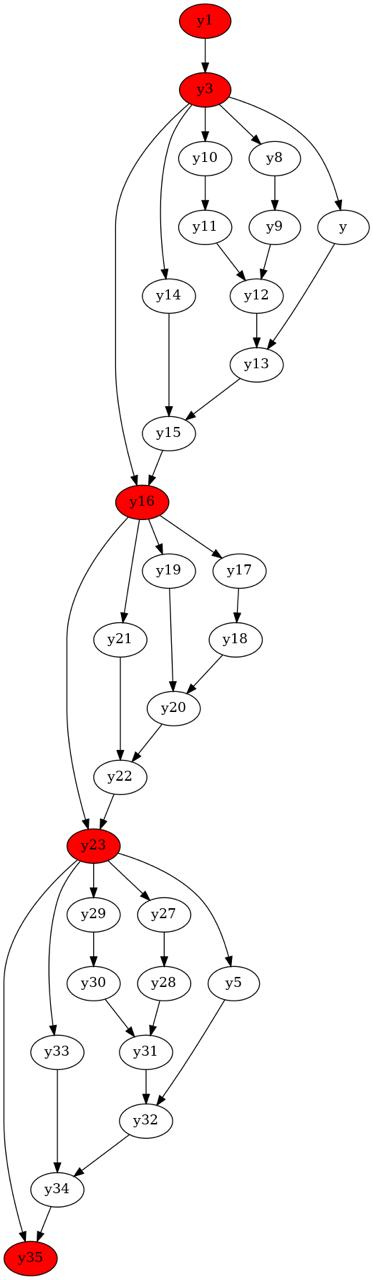
\includegraphics[width=0.9\linewidth]{graph_simple2.jpeg} 
    \caption{Simple}
    \end{subfigure}
    \begin{subfigure}{0.24\textwidth}
    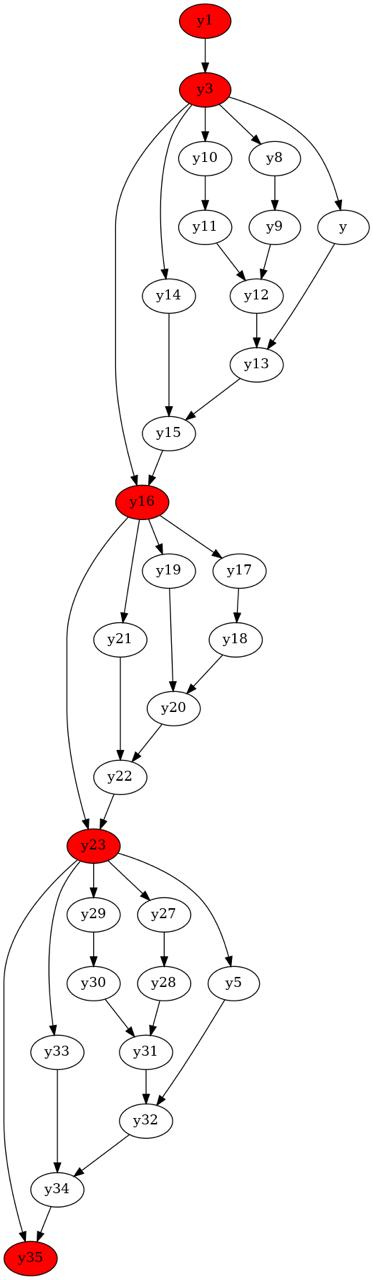
\includegraphics[width=0.9\linewidth]{graph_simple2.jpeg}
    \caption{Recursion}
    \end{subfigure}
    \begin{subfigure}{0.24\textwidth}
    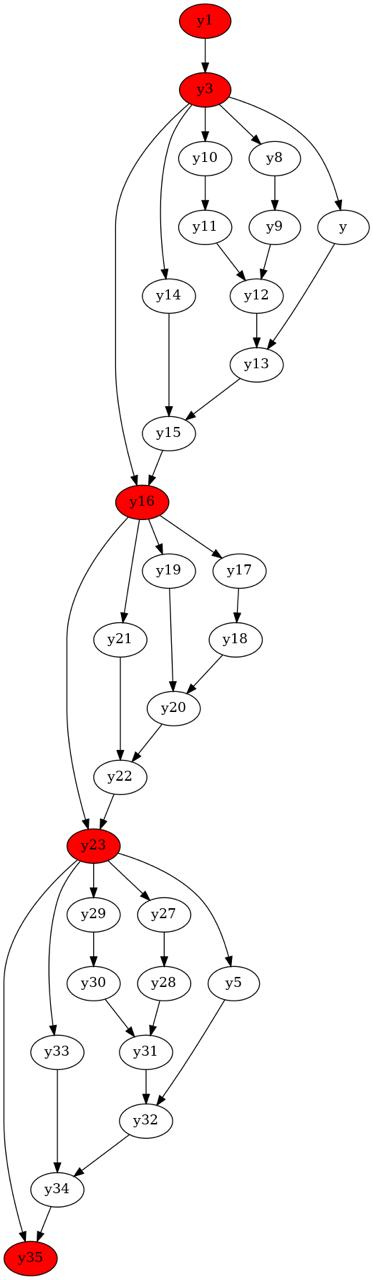
\includegraphics[width=0.9\linewidth]{graph_simple2.jpeg}
    \caption{If}
    \end{subfigure}
    \begin{subfigure}{0.24\textwidth}
    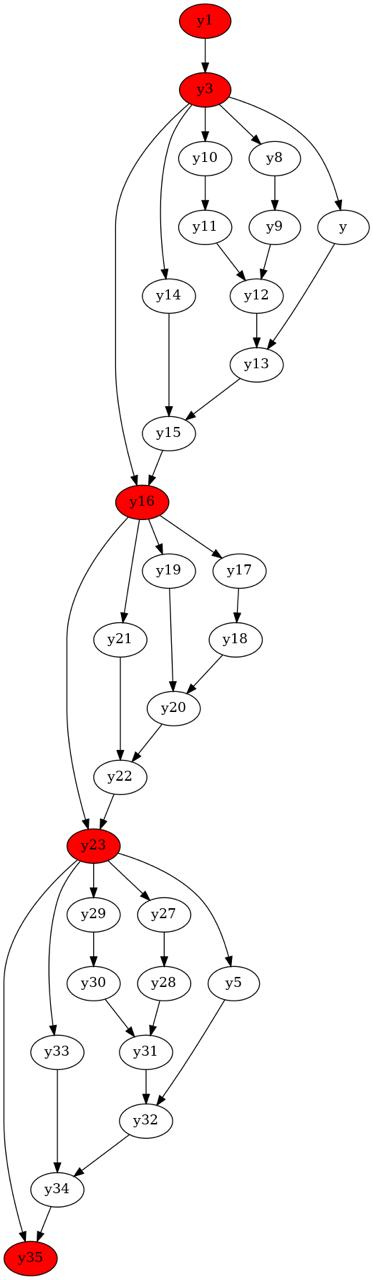
\includegraphics[width=0.9\linewidth]{graph_simple2.jpeg}
    \caption{IfAndRecursion}
    \end{subfigure}
    \captionsetup{justification = centering,
    singlelinecheck = false}
    \caption{Графовые виды различных систем уравнений}
    \label{all_graphs}
\end{figure}

С помощью изучения подобных графов было найдено несколько интересных с точки зрения оптимизации свойств. Так, оказалось, что около половины вершин имеют и входящую, и исходящую степень равную единице, то есть соответствующие $y_i$ используются только в одном $T_j$, а $T_i$ содержит только один $y_k$. В области графовых алгоритмов для уменьшения задачи применяют \textit{стягивание} таких вершин, то есть рёбра $u\rightarrow w$ и $w\rightarrow v$ заменяются на одно ребро $u\rightarrow v$, а вершина $w$ удаляется. Интерпретируя этот подход для системы уравнений, получим оптимизацию, которая заранее подставляет тела все стягиваемых уравнений, не вычисляя их, и удаляет соответствующие уравнения:

\begin{megaalgorithm}\captionsetup{labelfont={sc,bf}, labelsep=newline}
    \caption{contractions}
  \begin{algorithmic}
    \State $(Y, P)\gets$ input
    \State $T \gets P(y_0, y_n)$
    \For{$i \gets 1$ to $|Y|$}
        \If{$indeg(y_i) = 1$ and $outdeg(y_i) = 1$}
            \For{$j \gets i + 1$ to $n$}
                \State $T_j \gets T_j [y_i := T_i]$
            \EndFor
            \State $P \gets P [y_i := T_i]$
            \State $Y \gets Y \setminus (y_i, T_i)$
        \EndIf
    \EndFor
    \State \Return {$basic\_strategy(Y, P)$}
  \end{algorithmic}
\end{megaalgorithm}

Другим интересным наблюдением является тот факт, что подавляющее большинство вершин имеют исходящую степень, равную единице, то есть для большинства $y_i$ верно, что $y_i$ используется только в одном $T_j$. При подстановке таких $y_i$ может возникнуть дубликация, однако дальнейший анализ графов показывает, что эта дубликация не будет носить экспоненциальный характер. Вершины, имеющие исходяющую степень, большую чем один, разбивают граф на несколько блоков, при этом каждый блок содержит небольшое количество вершин. Таким образом, при стягивании вершин из такого блока, хоть дубликация и может возникнуть, но она не будет распространяться между блоками и приумножаться. Согласно этим соображениям, интересной для исследования является также оптимизация \texttt{contractions-strong}, заключающаяся в предварительной подстановка без редукции всех вершин, имеющих исходящую степень один.

\begin{megaalgorithm}\captionsetup{labelfont={sc,bf}, labelsep=newline}
    \caption{contractions-strong}
  \begin{algorithmic}
    \State $(Y, P)\gets$ input
    \For{$i \gets 1$ to $|Y|$}
        \If{\textcolor{red}{$outdeg(y_i) = 1$}}
            \For{$j \gets i + 1$ to $n$}
                \State $T_j \gets T_j [y_i := T_i]$
            \EndFor
            \State $P \gets P [y_i := T_i]$
            \State $Y\gets Y \setminus (y_i, T_i)$
        \EndIf
    \EndFor
    \State \Return {$basic\_strategy(Y, P)$}
  \end{algorithmic}
\end{megaalgorithm}

TODO

\subsection{Оптимизации, основанные на типах данных}\label{typebased}

В предыдущем разделе представлены две оптимизации, потенциально способных ускорить вычисления на данных, имеющих определённую структуру, и поставлен вопрос относительно их практической применимости в связи с накладными расходами на явное построение графа и вычисление степеней вершин. В этом разделе будут разработаны, апроксимирующие необходимые графовые свойства на основе типов данных.

Вернёмся к рисунку \ref{all_graphs} и обратим внимание на цвета вершин. Они соответствуют типам данных $y_i$ и обозначают следующие типы:

\begin{itemize}
    \item ?? вершины имеют тип \texttt{Ledger}, описывающий глобальное состояние системы. Этот тип включает в себя, помимо состояния глобальных переменных, также данные о других смарт-контрактах, балансах и конфигурации сети, поэтому данные такого типа как правило являются относительно большими термами.
    \item ?? вершины имеют тип \texttt{ControlResult} и связаны с порядком выполнения (control flow) программы, в том числе с такими конструкциями, как обработка ошибок и рекурсивный вызов функций.
    \item ?? вершины имеют тип \texttt{FieldType} и описывают проекции структур, то есть чтение отдельных полей у структур данных (в том числе, но не только, у глобального состояния типа \texttt{Ledger}).
    \item ?? вершины имеют тип \texttt{LocalStateMapping} и соответствуют получению информации о состоянии локальных переменных.
    \item Нераскрашенные вершины имеют пользовательские типы, соответствующие типам в исходной программе, например, численные или булевые.
\end{itemize}

В результате анализа графов были сформулированы следующие утверждения о соответствии типов вершин и их графовых свойствах:

\begin{enumerate}
    \item Все вершины типа \texttt{ControlResult} (??) имеют исходяшую степень, равную единице.
    \item Все вершины типа \texttt{LocalStateMapping} (??) и \texttt{FieldType} (??) имеют входящую и исходящую степень, равную единице.
    \item
    \item
\end{enumerate}

В случаях, где утверждается точные характеристики (а именно в утверждениях ??), эти утверждения также были установлены верными в результате анализа алгоритма построения системы уравнений и его реализации. 

\begin{megaalgorithm}\captionsetup{labelfont={sc,bf}, labelsep=newline}
    \caption{contractions-typebased}
  \begin{algorithmic}
    \State $(Y, P)\gets$ input
    \For{$i \gets 1$ to $|Y|$}
        \If{\textcolor{red}{$typeof(y_i)$ is $LocalStateMapping$ or $FieldType$}}
            \For{$j \gets i + 1$ to $n$}
                \State $T_j = T_j [y_i := T_i]$
            \EndFor
            \State $P \gets P [y_i := T_i]$
            \State $Y\gets Y \setminus (y_i, T_i)$
        \EndIf
    \EndFor
    \State \Return {$basic\_strategy(Y, P)$}
  \end{algorithmic}
\end{megaalgorithm} 

\begin{megaalgorithm}\captionsetup{labelfont={sc,bf}, labelsep=newline}
    \caption{contractions-strong-typebased}
  \begin{algorithmic}
    \State $(Y, P)\gets$ input
    \For{$i \gets 1$ to $|Y|$}
        \If{\textcolor{red}{$typeof(y_i)$ is not $Ledger$}}
            \For{$j \gets i + 1$ to $n$}
                \State $T_j \gets T_j [y_i := T_i]$
            \EndFor
            \State $P \gets P [y_i := T_i]$
            \State $Y\gets Y \setminus (y_i, T_i)$
        \EndIf
    \EndFor
    \State \Return {$basic\_strategy(Y, P)$}
  \end{algorithmic}
\end{megaalgorithm}  

\subsection{Работа с условными операторами}

TODO

\subsection{Выводы и результаты по главе}

Произведён анализ входных данных, и на основе этого анализа разработаны стратегии вычисления. Представлено четыре базовые стратегии:
\begin{itemize}
    \item \texttt{native}
    \item \texttt{bottomup-naive}
    \item \texttt{bottomup-reductions}
    \item \texttt{topdown}
\end{itemize}

Каждая из этих стратегий может применяться либо сама по себе, либо после предварительного использования одного из четырёх алгоритмов эвристического упрощения:
\begin{itemize}
    \item \texttt{contractions}
    \item \texttt{contractions-strong}
    \item \texttt{contractions-typebased}
    \item \texttt{contractions-strong-typebased}
\end{itemize}

Также каждая стратегия может использовать одну из двух нативных редукций, \texttt{cbv} или \texttt{lazy}. Таким образом, всего представлено $4 \cdot 5 \cdot 2 = 40$ стратегий. Все эти стратегии были реализованы на языке Ltac.

TODO выводы по разделу 2.5

\end{document}
